\chapter*{\hfill{}УСЛОВИЕ\hfill{}}
Необходимо промоделировать систему, состоящую из генератора памяти и обслуживающего аппарата. Генератор подаёт сообщения, распределённые по нормальному закону, они проходят в память и выбираются на обработку по закону из лабораторной работы \textnumero2. Количество заявок конечно и задано. Предусмотреть случай, когда обработанная заявка возвращается обратно в очередь. Необходимо определить оптимальную длину очереди, при которой не будет потерянных сообщений. Реализовать, используя пошаговый и событийные подходы.

\chapter{Теоретическая часть}

\section{Равномерное распределение}

Непрерывное равномерное распределение~--- распределение случайной вещественной величины, принимающей значения, принадлежащие некоторому промежутку конечной длины, характеризующееся тем, что плотность вероятности на этом промежутке почти всюду постоянна.

Плотность распределения представлена в формуле \ref{eq:uniform_density}.

\begin{equation}\label{eq:uniform_density}
    f_X (x) =
    \begin{cases}
        \frac{1}{b-a}, x \in [a,b] \\
        0, x \notin [a, b] \\
    \end{cases}
\end{equation}

Функция распределения представлена в формуле \ref{eq:uniform_function}.

\begin{equation}\label{eq:uniform_function}
    F_X (x) =
    \begin{cases}
        0, x < a \\
        \frac{x - a}{b - a}, a \le x < b \\
        1, x \geq b \\
    \end{cases}
\end{equation}

\section{Нормальное распределение}

Нормальное распределение~--- распределение вероятностей, которое в одномерном случае задаётся функцией плотности вероятности, совпадающей с функцией Гаусса.

Плотность распределения представлена в формуле \ref{eq:gauss_density}.

\begin{equation}\label{eq:gauss_density}
    f_X (x) = \frac{1}{\sigma \sqrt{2 \pi}} e^{-\frac{(x - \mu)^2}{2 \sigma^2}}
\end{equation}

Функция распределения представлена в формуле \ref{eq:gauss_function}.

\begin{equation}\label{eq:gauss_function}
    F (x) = \frac{1}{\sigma \sqrt{2\pi}} \int_{-\infty}^x e^{-\frac{(t- \mu)^2}{2 \sigma^2}} dt
\end{equation}

\section{Пошаговый подход}
Пошаговый подход заключается в последовательном анализе состояний всех блоков в момент $t + \Delta t$ по заданному состоянию блоков в момент $t$. При этом новое состояние блоков определяется в соответствии с их алгоритмическим описанием с учетом действующих случайных факторов, задаваемых распределениями вероятности. В результате такого анализа принимается решение о том, какие общесистемные события должны имитироваться программной моделью на данный момент времени.

Основной недостаток этого подхода: значительные затраты машинного времени на реализацию моделирования системы. А при недостаточно малом $\Delta t$ появляется опасность пропуска отдельных событий в системе, что исключает возможность получения адекватных результатов при моделировании.

Достоинство: равномерная протяжка времени.

\section{Событийный подход}
Характерное свойство моделируемых систем~--- состояние отдельных устройств изменяется в дискретные моменты времени, которые совпадают с моментами поступления сообщений в систему, моментами окончания решения задач, моментами возникающих аварийных сигналов и т.д. Поэтому, моделирование и продвижение текущего времени в системе удобно проводить использую событийный принцип, при котором состояние всех блоков системы анализируется лишь в момент наступления какого-либо события. Момент наступления следующего события определяется минимальным значением из списка будущих событий, представляющих собой совокупность моментов ближайшего изменения состояний каждого из блоков системы.

\chapter{Примеры работы}

\begin{figure}[H]
    \centering
    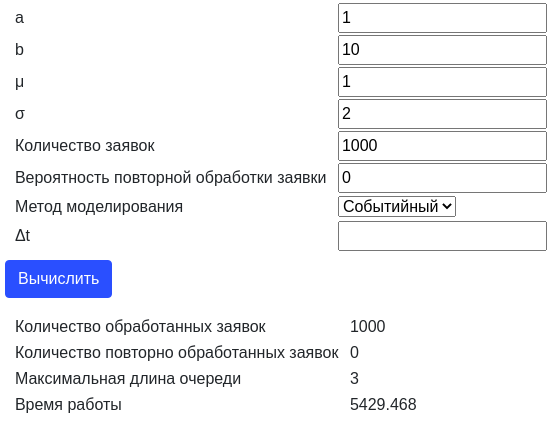
\includegraphics[width=0.6\textwidth]{images/scr01.png}
    \caption{Событийный подход, вероятность возврата заявки в очередь равна 0}
\end{figure}
\begin{figure}[H]
    \centering
    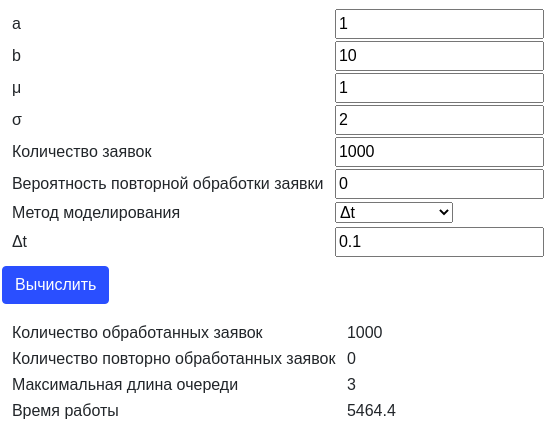
\includegraphics[width=0.6\textwidth]{images/scr02.png}
    \caption{Пошаговый подход, вероятность возврата заявки в очередь равна 0}
\end{figure}

\begin{figure}[H]
    \centering
    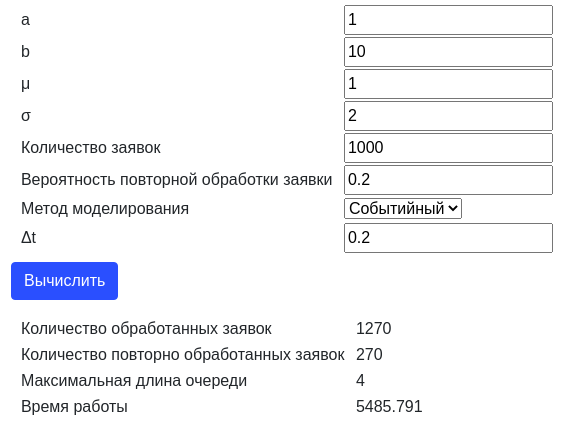
\includegraphics[width=0.6\textwidth]{images/scr03.png}
    \caption{Событийный подход, вероятность возврата заявки в очередь равна 0.2}
\end{figure}
\begin{figure}[H]
    \centering
    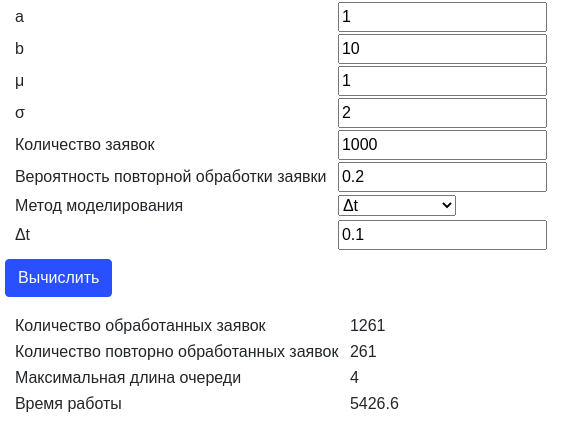
\includegraphics[width=0.6\textwidth]{images/scr04.png}
    \caption{Пошаговый подход, вероятность возврата заявки в очередь равна 0.2}
\end{figure}

\begin{figure}[H]
    \centering
    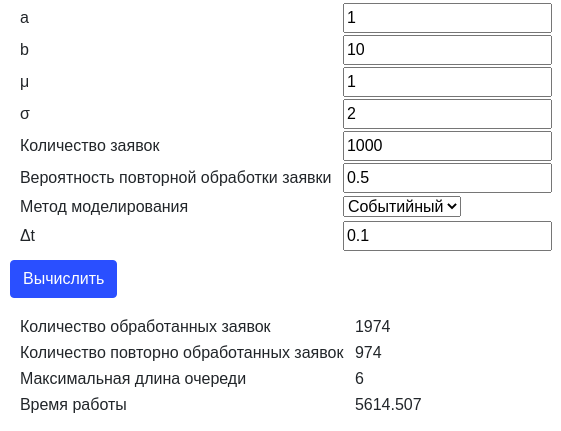
\includegraphics[width=0.6\textwidth]{images/scr05.png}
    \caption{Событийный подход, вероятность возврата заявки в очередь равна 0.5}
\end{figure}
\begin{figure}[H]
    \centering
    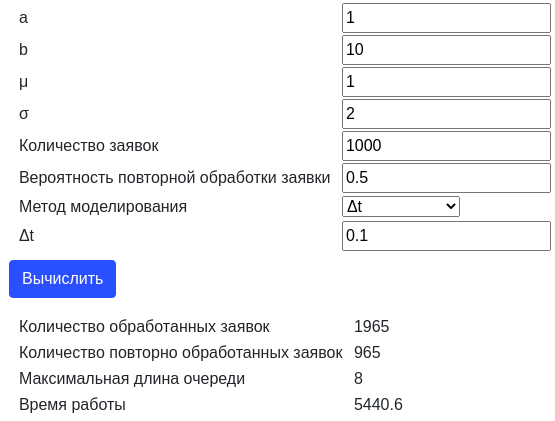
\includegraphics[width=0.6\textwidth]{images/scr06.png}
    \caption{Пошаговый подход, вероятность возврата заявки в очередь равна 0.5}
\end{figure}

\begin{figure}[H]
    \centering
    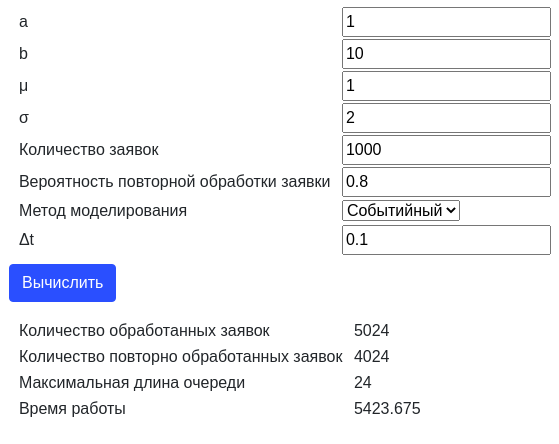
\includegraphics[width=0.6\textwidth]{images/scr07.png}
    \caption{Событийный подход, вероятность возврата заявки в очередь равна 0.8}
\end{figure}
\begin{figure}[H]
    \centering
    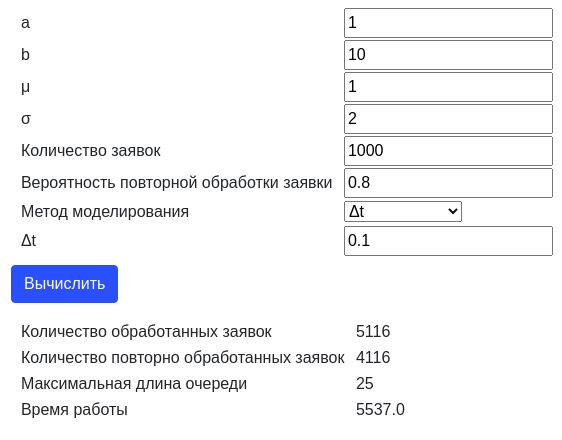
\includegraphics[width=0.6\textwidth]{images/scr08.png}
    \caption{Пошаговый подход, вероятность возврата заявки в очередь равна 0.8}
\end{figure}

\begin{figure}[H]
    \centering
    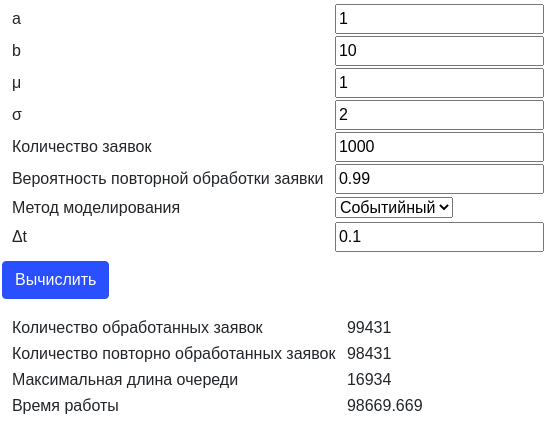
\includegraphics[width=0.6\textwidth]{images/scr09.png}
    \caption{Событийный подход, вероятность возврата заявки в очередь равна 0.99}
\end{figure}
\begin{figure}[H]
    \centering
    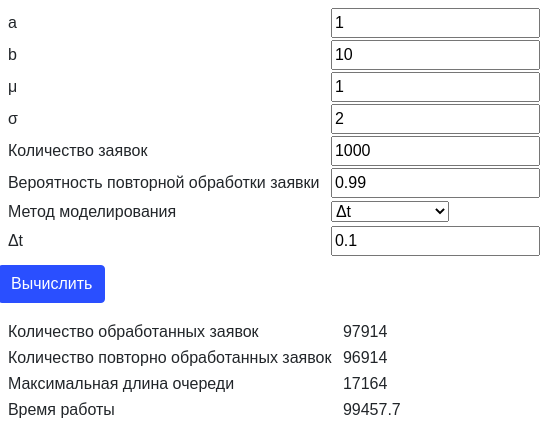
\includegraphics[width=0.6\textwidth]{images/scr10.png}
    \caption{Пошаговый подход, вероятность возврата заявки в очередь равна 0.99}
\end{figure}
